\section{Entropy}

\subsection{Types of Systems}

Just before we define our notion of this mysterious "entropy", it will help to define what different kinds of systems mean. An \textbf{Open system} is one in which both matter and energy can be exchanged with its environment. A \textbf{Closed system} is a system where energy can be exchanged with the environment, but no matter. Finally, an \textbf{isolated} system is where neither matter nor energy can be exchanged with the environment. \\

As a quick example, suppose the system is a half cup of water. If we leave the top of the cup open, it's an open system as the water molecules can evaporate and leave the cup. If we close the top of the cup, then it's a closed system as we can still give energy to the cup (say, by heating it in a microwave) even if the water molecules can't escape from it. If the cup is perfectly insulated and closed off, then its an isolated system as neither matter nor energy can enter or exit the cup.

\subsection{Entropy and Second Law of Thermodynamics}

We saw that interacting systems, after long time, reach thermal equilibrium when they are in the macrostate with the greatest multiplicity. This is the result of the \textbf{second law of thermodynamics}: multiplicity tends to increase. \\

In order to quantify multiplicity, we define entropy:

\[ S=k_B\ln\Omega \]

It is nothing but the scaled natural logarithm of the number of microstates of the system in some particular macrostate $\Omega$. The reason we take logarithm of $\Omega$ is that $\Omega$ tends to be very large. Logarithm helps us to easily perform calculations involving large numbers. \\

Sometimes entropy is defined as the amount of ``disorder'' in the system but this definition is ambigious and is hard to quantitfy. It is best to think entropy as the amount of microscopic information we don’t have access to. $S(U,V,N)$ counts the number of missing information with just three state variables to describe the large system of $N$ particles. There really is no macroscopic variable that determines the configuration (positions, velocities) of all the particles. The second law of thermodynamics says that we are continually losing information about the microstates in the universe. We can’t gain microscopic information from macroscopic measurements or manipulations. \\

A ``missing information'' function can be written in terms of the probabilities of sampling the possible microstates of the system:

\[S(\{p_i\})=-\sum_{i=1}^\Omega p_i \ln(p_i)\]

This is known as the Shannon entropy. \\

So for a deck of cards, for example, if you just unwrapped it, there is a particular order of the cards that you could be certain of, out of the $52!$ possibibities. There is no missing information and the system is in one particular state. Here, one of the states has probability $1$, and all the others have probability $0$. The Shannon entropy in this case is:

\[S=-1\ln(1)-\sum_{i\ne1}0\ln(0)=0\]

Now suppose if all states are equally likely, the entropy becomes:

\begin{align*}
	S&=-\sum_{i=1}^\Omega \frac{1}{\Omega} \ln\left( \frac{1}{\Omega} \right) \\
	&=-\frac{1}{\Omega} \ln\left( \frac{1}{\Omega} \right) \sum_{i=1}^\Omega 1 \\
	&=\frac{1}{\Omega} \ln\left( \Omega \right) \Omega \\
	&=\ln\left( \Omega \right)
\end{align*}

This looks similar to the entropy we defined earlier! \\

The total entropy of a composite system containing two parts $A$ and $B$ is the sum of entropies of $A$ and $B$:

\[S_{total}=k_B\ln\Omega_{total}=k_B\ln(\Omega_A\Omega_B)=k_B\ln\Omega_A+k_B\ln\Omega_B=S_A+S_B\]

This result can be generalized to system containing more than two parts. We also see another reason to take logarithm of $\Omega$. Recall from last section that $\Omega$ is a ``super extensive'' quantity. We take logarithm of $\Omega$ in order to turn it into a quantity which can be added up linearly. This makes the logarithm of $\Omega$ (a.k.a entropy) an extensive quantity! \\

Entropy is a physical property of a system at equilibrium, like internal energy and enthalpy. It measures how internal energy is distributed among the molecules of the system. In general, the more particles there are in a system, the bigger the system is, and the more energy it contains, the greater its entropy and multiplicity. \\

There is more precise statement for the second law of thermodynamics. The total entropy of an \textit{isolated} system either increases or remains constant in any \textbf{spontaneous process}\footnote{Spontaneous processes refers to a process in which a system evolute in time without any external input. The evolution makes the system reach to its thermal equilibrium. An example of such process is a dispersion of gas molecules in a sealed container.}, but it never decreases\footnote{Actually, it is possible for entropy of an isolated system to decrease. Flucation theorem says that there is always some nonzero probability that entropy spontaneously decrease.}. The second law explains why heat can only flow spontaneously from the hot object to the cold object, but not not the other way around because it will decrease entropy. \\

For open or closed systems, it is more preferrable to rewrite the second law mathematically as follows:

\[ \Delta S_{univ} = \Delta S_{sys} + \Delta S_{surr} \ge 0 \]

The total entropy change in the universe is the sum of the entropy changes in its independent quantities: the system and its surroundings. The total entropy of the universe either must increase or stay constant. A decrease in system entropy can only occur spontaneously if the entropy change of the surroundings is both positive in sign and has a larger magnitude than the entropy change of the system:

\[\Delta S_{surr} > 0\]

and

\[\left|\Delta S_{surr}\right| > \left|\Delta S_{sys}\right|\]

One possible situation when entropy decreases sponteneously is the freezing of a cup of water in below freezing temperatures\footnote{Whether a process is spontaneous or not depends a given set of conditions. In the case of water freezing at below freezing temperatures, it’s irreversible because at below freezing temperatures and you can never observe water melting. It’s spontaneous because it’s the natural process that happens and leads to entropy production.}. \\

Let's study an isolated system made up of two components: $A$ and $B$. The total energy $U_{tot}+U_A+U_B$ is constant. The only macroscopic internal adjustment the system can make is to move energy between $A$ and $B$. The macrostates are described by $U_A$ alone.

\begin{figure}[H]
	\centering
	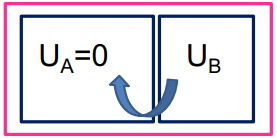
\includegraphics[width=100mm]{32.png}
\end{figure}

Suppose we start with $U_A=0$. Since system $A$ has zero energy, it has one possible microstate, so that means its initial entropy is zero: $S=k_B\ln1=0$. On the other hand, system $B$ has energy $U_B=U_{tot}-U_A$. It has higher entropy than system $A$. This means energy will spontaneously flow from system $B$ to system. By the second law of thermodynamics, entropy of system $A$ will increase while the entropy of system $B$ will decrease.

\begin{figure}[H]
	\centering
	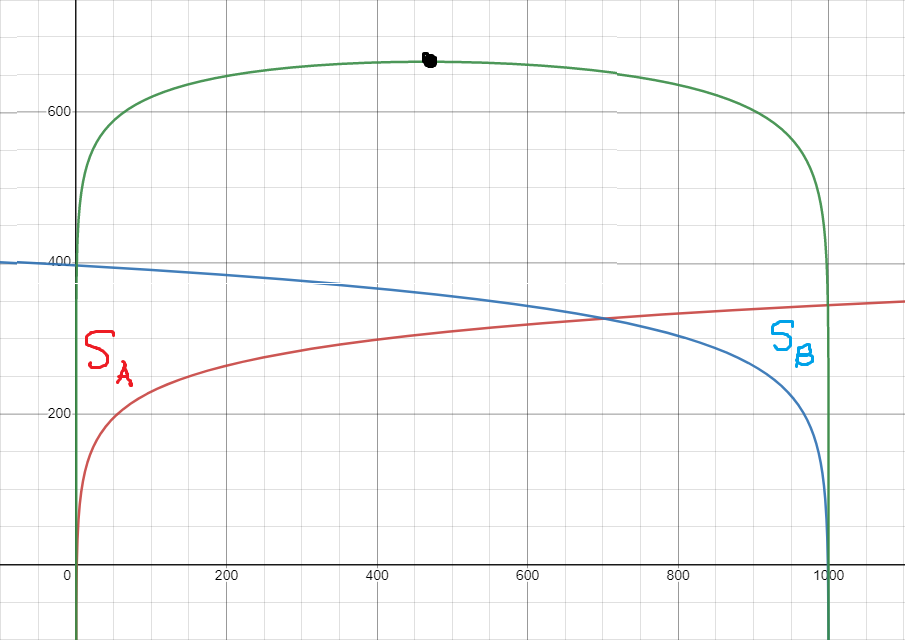
\includegraphics[width=100mm]{33.png}
	\caption{Graphs of $S$, $S_A$ and $S_B$ when $U_{tot}=1000$ (\href{https://www.desmos.com/calculator/px64pose4a}{Desmos link}). Black dot is the equilibrium point}
\end{figure}

From the graph above, we see that the increasing of system $A$'s entropy is faster than the decreasing of system $B$'s entropy:

\[|\Delta S_A|>|\Delta S_B|\]

since the slope for the $S_A$ curve is steeper than the slope for the $S_B$ curve. The total entropy of the isolated system $S$ will spontaneously keep increasing until thermal equilibrium (at $U_A=465$) is reached where it will remain constant. At thermal equilibrium,

\[\frac{\partial S}{\partial U_A}=0\]

\[\frac{\partial S_A}{\partial U_A}=\frac{\partial S_B}{\partial U_B}\]

Recall from last unit that at equilibrium, temperatures of $A$ and $B$ are equal. Also, we defined inverse temperature $\beta$ as:

\[\beta=\frac{\partial \ln\Omega}{\partial U}\]

Let's redefine temperature in terms of entropy. Since $\beta=\frac{1}{k_BT}$,

\[\frac{1}{k_BT}=\frac{\partial \ln\Omega}{\partial U}\]
\[\frac{1}{T}=\frac{\partial k_B\ln\Omega}{\partial U}=\frac{\partial S}{\partial U}\]

Finally,

\[\boxed{\frac{1}{T}=\left(\frac{\partial S}{\partial U}\right)_{N,V}}\]

or

\[\boxed{T=\left(\frac{\partial U}{\partial S}\right)_{N,V}}\]

Temperature of a system is the reciprocal of the slope of its entropy vs. energy graph. The partial derivative is computed with the system's volume and number of particles treated as constant. \\

This new definition of temperature allows us to find a formula for measuring entropy changes. Suppose we add a bit of heat $\delta Q$ to a system while holding its volume $V$ and the number of particles $N$ constant and doing no other forms of work, the first law of thermodynamics says:

\[\Delta U=\delta Q\]

The change in entropy can be approximated using:

\[\Delta S=\left(\frac{\partial S}{\partial U}\right)_{N,V} \Delta U=\frac{\delta Q}{T}\]

assuming that temperature is kept constant during the process. But in the real world, temperature is not always constant, so we need to consider an infinitesimal change in entropy:

\[dS=\frac{\delta Q_{rev}}{T}\]

This is the classical definition of entropy. Entropy is a state function. Recall that any change in any thermodynamic state function is always independent of the path taken. The type of path depends on whether the process is reversible or not. \\

A physical process that increases the total entropy of the universe $\Delta S_{univ}>0$ cannot happen in reverse, as it would violate the second law of thermodynamics. They are called \textbf{irreversible process}. Examples include, paper getting burned, boiling of water, and the sun warming up Earth surface. Spontaneous processes are irreversible because they happen naturally on their own. \\

On the other hand, a process that leaves the total entropy of the universe unchanged $\Delta S_{univ}=0$ are said to be reversible. If the total entropy is $S_{univ} = S_{sys}+S_{surr}$, then for reversible processes,

\[\Delta S_{sys} = -\Delta S_{surr}\]

\begin{texample}
	Heat flows from a body at temperature $T$ to a body at temperature $T-dT$ , where $dT$ is small. A slight warming up of the second body, by $2dT$, reverses the direction of heat flow. Show that the total entropy remains unchanged. \\
	
	The total entropy change is:
	
	\[dS=-\frac{\delta Q}{T}+\frac{\delta Q}{T-dT}\]
	
	Since $\delta Q=CdT$,
	
	\begin{align*}
		dS&=CdT\left( \frac{1}{T-dT}-\frac{1}{T} \right) \\
		&=\frac{CdT}{T}\left( \frac{1}{1-\frac{dT}{T}}-1 \right)
		\intertext{Applying Taylor's expansion for $\frac{1}{1-x}$,}
		&=\frac{CdT}{T}\left( 1+\frac{dT}{T}-1 \right) \\
		&=C\frac{dT^2}{T^2}
	\end{align*}
	
	We see that $dS\sim O(dT^2)\to0$.
\end{texample}

In principle, no macroscopic process is perfectly reversible, although in practice, some processes come close enough. Reversible processes must happen \textbf{quasistatically} (ie. happens so slowly that the system under consideration remains arbitrarily close to equilibrium (with itself) at all times). For example, when the gas is compressed slowly so that there is (nearly) uniform pressure and temperature inside (ie. the intensive variables are constant throughout the system), the quantum mechanical wavefunction of gas molecules has energies of all the levels increase. But molecules will not be promoted into higher energy levels since it is a quasistatic process. A molecule that starts in $n$th level (although the energy of that level increases), will stay at $n$th level after slow compression.

\begin{figure}[H]
	\centering
	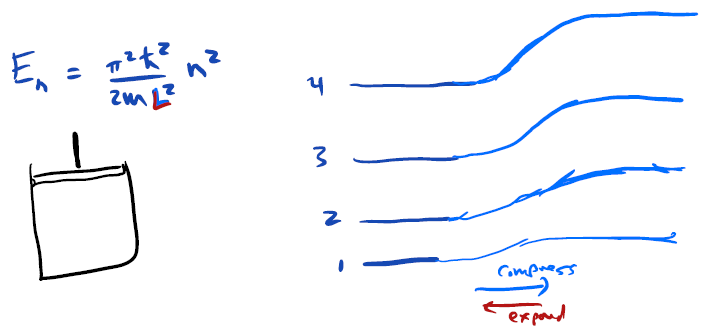
\includegraphics[width=100mm]{34.png}
	\caption{Gas Compression and its Energy Levels}
\end{figure}

Hence, the number of ways of arranging the molecules among the various energy levels will remain the same, so entropy does not change. On the other hand, if the compression is violent enough to kick molecules up into higher levels, then the number of possible arrangements will increase and so will the entropy. \\

This means reversible processes often occurr microscopically when a system is at thermal equilibrium with its surroundings. This causes us to define all our reversible processes (and entropy) as infinitesimals. In fact, no reversible process actually exists on a macroscopic scale. \\

As an example of why this is, let's take a look at a process that is theoretically reversible, but isn't actually reversible. Say we have a container of a gas with a piston on one face, but insulated such that it cannot exchange heat (or molecules) with its environment. However, it is connected to a neighbouring infinitely large heat bath, where it can exchange heat with (but not molecules).

\begin{figure}[H]
	\centering
	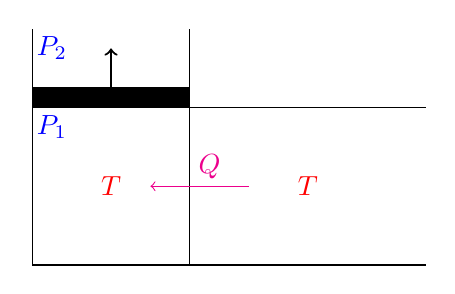
\begin{tikzpicture}
		\draw[draw=black] (0,0) rectangle (2,2);
		\draw[fill = black] (0,2) rectangle (2,2.25);
		\draw (0,2) -- (0,3);
		\draw (2,2) -- (2,3);
		\draw (2,2) -- (5,2);
		\draw (2,0) -- (5,0);
		\draw[->, thick] (1, 2.25) -- (1, 2.75);
		\draw[text=blue] (0.25,1.75) node {$P_1$};
		\draw[text=blue] (0.25, 2.75) node {$P_2$};
		\draw[text=red] (1,1) node {$T$};
		\draw[text=red] (3.5,1) node {$T$};
		\draw[magenta, ->] (2.75,1) -- (1.5,1);
		\draw[text=magenta] (2.25, 1.25) node {$Q$};
	\end{tikzpicture}
	\caption{Piston with infinite heat bath to the right.}
\end{figure}

In this situation, we have that $P_{1}>P_{2}$, so the piston will undergo an expansion. Since the heat bath beside it will keep it at the same temperature, the expansion will be isothermal. So since the temperature of the two sides of the piston/heat bath barrier is constant and equal, the heat transfer across it reversible right? Well, not quite. And it has to do with the idea that a perfectly isothermal process doesn't exist either. \\

To figure out why, let's break down what happens step by step. Initially, both the gas and the heat bath are at the same temperature, so no net heat flow between them. However, the pressure inside the piston is greater than the pressure outside. So the piston expands. When it does this, it does work on the environment, and loses energy. This in turn causes its temperature to fall. Its temperature dropping causes heat to flow spontaneously across from the heat bath, until the gas returns to its original temperature. Rinse, repeat until the internal and external pressures are equal. \\

So we can see that during an isothermal process, the temperature isn't quite constant. However, if we do this process \textit{very} slowly, the heat flow will manage to restore the temperature so quickly (or to put it another way, heat will flow into the system much faster than the system does work) that the temperature be \textit{almost} constant the whole time. This is what we really mean by an isothermal process. It's also why entropy is defined infinitesimally since we approximate that each of our tiny expansion steps of the piston happen at constant temperature. \\

Let's revisit the classical definition of entropy. $\delta Q_{rev}$ represents the infinitesimal amount of spontaneous reversible heat flow that occurs during the process. The heat flow must very tiny so that it has an equal chance of happening in both directions: from hot to cold and from cold to hot. $T$ is the temperature of either the system \textbf{or} the surroundings at the instant of the infinitesimal change. The subscript $rev$ indicates that while heat flow is path-dependent, entropy change is not. \\

For a reversible process, the entropy change of the system and the surroundings are equal and opposite at any step. We need only calculate one or the other. The sum $\Delta S_{sys}+\Delta S_{surr}$ is zero. Hence the statement that a reversible process results in $\Delta S_{univ}=0$ always. This means, we only need to know one or the other, not both. \\

We can and will always evaluate the (infinitesimal) entropy change of a system $dS_{sys}$ by choosing a reversible process. For an irreversible process, we need to define the exact status of the universe when we propose that a system will undergo an irreversible process. The closer the system and the surroundings are to being at exact thermodynamic equilibrium during the proposed process, the smaller will be the irreversibility of the process that occurs.. The magnitude of the irreversible entropy change for any process depends on the magnitude of the difference between the system and the surroundings from exact thermodynamic equilibrium. So, if extra entropy is generated $\Delta S_{univ}\ge0$, the process is irreversible. \\

For reversible processes, $dS=\frac{\delta Q}{T}$ and for irreversible processes, $dS>\frac{\delta Q}{T}$. To see why the latter is true, consider a gas in piston cylinder. Suppose we hit the piston very hard so that it compresses the gas really fast by some very small amount. Let $P_i$ and $P_f$ be the pressure before and after this compression. After compression, the pressure is initially very high but it will later settle down so that the pressure has only increased infinitesimally $P_f\approx P_i$. The overall work done in this process is $W>-P_fdV$\footnote{$dV$ is negative, so $W$ is positive.}\footnote{If the compression is instead done quasistatically, $-P_idV<W<-P_fdV$ or $W\approx -P_{ave}dV$.}. According to the first law of thermodynamics\footnote{Or the first thermodynamic identity which we will see in the next section.}, $Q<TdS$. This means $dS>\frac{\delta Q}{T}$. Extra entropy is created in irreversible processes. \\

So, the change of entropy always satisfies the following inequality:

\[dS \geq \frac{\delta Q}{T}\]

for all processes. \\

Suppose we have two bodies in a brief thermal contact with each other: $A$ and $B$. The temperatures of the bodies are $T_A$ and $T_B$ respectively and $T_A>T_B$. To calculate the total entropy change when heat $Q$ leaves body $A$ and flow into body $B$, assuming that the bodies are massive (or heat transferred $Q$ is small):

\[\Delta S_{tot}=\frac{-Q}{T_A}+\frac{+Q}{T_B}\]

The body $A$ has its entropy decreased while the body $B$ has its entropy increased. So, for all $T_A>T_B$, $\Delta S_{tot}>0$. As the two temperatures get closer and closer to each other, $\Delta S_{tot}$ goes to $0$. Entropy increases as heat gets transferred which makes heat transfers irreversible processes. Note that spontaneous transfer of heat from body $B$ to $A$ is forbidden because it will make $\Delta S_{tot}<0$ which violates the second law of thermodynamics.

\begin{texample}
	An object with temperature $T_H=\SI{400}{\kelvin}$ is placed briefly in thermal contact with a cooler object at temperature $T_C=\SI{300}{\kelvin}$. A small amount of heat $\SI{1200}{\joule}$ flows between the two objects. How much has the entropy of the world changed? \\
	
	The heat will flow from the hotter object to the colder object. The total entropy change is the sum of entropy changes for both objects:
	
	\[\Delta S=\Delta S_H+\Delta S_C=\frac{Q_H}{T_H}+\frac{Q_C}{T_C}\]
	
	where $Q_H$ is the amount of heat flowed \textit{in} the hot object which is negative in this question and $Q_C$ is the amount of the heat flowed in the cold object.
	
	\[\Delta S=\frac{-\SI{1200}{\joule}}{\SI{400}{\kelvin}}+\frac{+\SI{1200}{\joule}}{\SI{300}{\kelvin}}=\SI{1}{\joule\per\kelvin}\]
\end{texample}

If the temperature is instead varying, the total entropy should take account of varying temperature. Also, we use $Q=C_vdT$ to express the relationship in terms of constant volume heat capacity:

\[dS=\frac{C_vdT}{T}\]

The total change in entropy can be calculated by integration:

\[\Delta S=\int dS=\int_{T_i}^{T_f} \frac{C_v}{T} dT\]

\begin{texample}
	A steel ball with heat capacity $C_v=\SI{1000}{\joule\per\kelvin}$ is being warmed by the heat of the Sun. Its temperature increases from $\SI{300}{\kelvin}$ to $\SI{350}{\kelvin}$. How much does its entropy change? Assume $C_v$ is constant. \\
	
	\begin{align*}
		\Delta S&=\int_{T_i}^{T_f} \frac{C_v}{T} dT \\
		&=C_v \ln\left( \frac{T_2}{T_1} \right) \\
		&=\SI{1000}{\joule\per\kelvin} \ln\left( \frac{350}{300} \right) \\
		&=\SI{154}{\joule\per\kelvin}
	\end{align*}
\end{texample}

\begin{texample}
	An ice cube (mass $\SI{10}{\gram}$) at zero degree Celsius is left stting on the kitchen table, where it gradually melts. The temperature in the kitchen is $\SI{25}{\celsius}$. Calculate the net change in the entropy of the universe during the entire melting process (assuming that the volume is constant). \\
	
	The latent heat for melting ice is $l=\SI{333}{\joule\per\gram}$. The heat capacity of water is $c=\SI{4.18}{\joule\per\kelvin\per\gram}$. \\
	
	The change in the entropy of the ice cube as it melts into water at zero degree Celsius is:
	
	\[\Delta S_{ice}=\frac{Q}{T}=\frac{l (\SI{10}{\gram})}{\SI{273}{\kelvin}}=\SI{12.2}{\joule\per\kelvin}\]
	
	The heat capacity is $C_v=c (\SI{10}{\gram})=\SI{41.8}{\joule\per\kelvin}$. The change in the entropy of the water (from the melted ice) as its temperature rises from zero to $\SI{25}{\celsius}$ is:
	
	\[\Delta S_{water}=\int_{T_i}^{T_f} \frac{C_v}{T}dT=C_v \ln\left(\frac{T_f}{T_i}\right)=(\SI{41.8}{\joule\per\kelvin}) \ln\left( \frac{298.15}{273.15} \right)=\SI{3.66}{\joule\per\kelvin}\]
	
	The total heat lost from the kitchen is the amount of heat required to melt ice into water:
	
	\[Q_{tot}=l (\SI{10}{\gram})+C_v (\SI{298.15}{\kelvin}-\SI{273.15}{\kelvin})=\SI{4375}{\joule}\]
	
	Since the kitchen acts as a heat bath, its temperature is constant. The entropy loss by the kitchen is:
	
	\[\Delta S_{kitchen}=\frac{-Q_{tot}}{T}=\frac{-\SI{4375}{\joule}}{\SI{298.15}{\kelvin}}=-\SI{14.67}{\joule\per\kelvin}\]
	
	The overall entropy increase is:
	
	\[\Delta S_{univ}=\Delta S_{ice}+\Delta S_{water}+\Delta S_{kitchen}=\SI{1.18}{\joule\per\kelvin}\]
	
	as expected.
\end{texample}

\begin{texample}
	In order to take a nice warm bath, you mix $\SI{55}{\liter}$ of hot water at $65$ degrees celsius, with $\SI{20}{\liter}$ of cold water at $10$ degrees celsius. How much new entropy have you created by mixing the water? \\
	
	The volume heat capacity for hot water is $C_h=\SI{4.18}{\joule\per\kelvin\per\gram} (\SI{55000}{\gram})=\SI{229900}{\joule\per\kelvin}$ and for cold water: $C_{c}=\SI{4.18}{\joule\per\kelvin\per\gram} (\SI{20000}{\gram})=\SI{83600}{\joule\per\kelvin}$. \\
	
	Conservation of energy will give the final temperature of the bath.
	
	\[\Delta U=C_{h}(T_F-T_h)+C_{c}(T_F-T_c)=0\]
	
	where $T_h=\SI{338.15}{\kelvin}$ and $T_c=\SI{283.15}{\kelvin}$. This gives $T_F=\SI{323.5}{\kelvin}$. \\
	
	The change of entropies are:
	
	\[\Delta S_{h}=\int_{T_h}^{T_F} \frac{C_h}{T}dT=-\SI{10182}{\joule\per\kelvin}\]
	\[\Delta S_{c}=\int_{T_c}^{T_F} \frac{C_c}{T}dT=\SI{11137}{\joule\per\kelvin}\]
	
	The total entropy change of the universe is:
	
	\[\Delta S_{univ}=\Delta S_{h}+\Delta S_{c}=\SI{955}{\joule\per\kelvin}\]
\end{texample}

\subsection{First Thermodynamic Identity}

There is the relationship between internal energy, temperature, pressure and entropy. But before we start, let's derive the relationship between pressure and internal energy. Consider an arbitrary system (gas, for example) sits inside an \textit{insulated} container, with an adjustable heavy piston that is well-balanced by some weights. Let friction be negligible. By adding a bit of mass to either the hanging weight, or on top of the piston, we can quasistaticaly adjust the volume inside the container, making it a bit larger or smaller, respectively.

\begin{figure}[H]
	\centering
	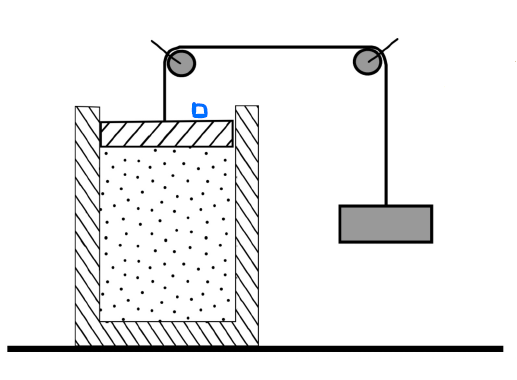
\includegraphics[width=100mm]{35.png}
	\caption{Gas in Piston}
\end{figure}

Since the gas is insulated from the surroundings, heat cannot escape, so $Q=0$. According to the first law of thermodynamics:

\[dU_{sys}=\delta W_{on}=-P_{sys} dV_{sys}\]

The process is quasistatic, so $\Delta S_{univ}=\Delta S_{sys}=0$\footnote{This makes it an \textit{isentropic} process, since both change in entropy and heat is zero}. Also, the amount of the particles in gas is kept constant. The relationship between pressure and internal energy is:

\[\boxed{P=-\left( \frac{\partial U}{\partial V} \right)_{S,N}}\]

This relationship will also be handy:

\[T=\left( \frac{\partial U}{\partial S} \right)_{V,N}\]

We now have everything in place to find the relationship between internal energy, temperature, pressure and entropy. Imagine a two-step process, where we change the state of the system so that $S\to S+\Delta S$ at constant volume, and then we let $V\to V+\Delta V$ at constant entropy.

\begin{figure}[H]
	\centering
	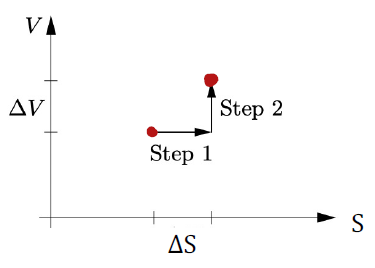
\includegraphics[width=100mm]{36.png}
	\caption{Two-Step Process}
\end{figure}

Assuming that $\Delta S$ and $\Delta V$ are infinitesimal, the total change in internal energy is the sum of the changes in steps $1$ and $2$. We can write $dU$ as total differential:

\begin{align*}
	dU&=dU_1+dU_2 \\
	&=\left( \frac{\partial U}{\partial S} \right)_{V,N} dS+\left( \frac{\partial U}{\partial V} \right)_{S,N} dV \\
	&=TdS-PdV
\end{align*}

We derived the first thermodynamic identity:

\[\boxed{dU=TdS-PdV}\]

assuming that the number of particles in the system $N$ is fixed\footnote{If $N$ is varying, we need to add the extra term $\mu dN$ where $\mu$ is the chemical potential.}. This thermodynamic identity holds true for any infinitesimal change (ie. $P_f\approx P_i$ and $T_f\approx T_i$) in a system so long at the pressure and temperature are well-defined. The system is assumed to be in thermal equilibrium at the beginning and at the end of the process (ie. the whole process is quasistatic) so that state functions (such as energy, pressure, temperature) are well defined\footnote{A system that is not in thermal equilibrium might be one where one side of system is hotter than the other: clearly we cannot really speak of a true temperature}. \\

We say a thermodynamic variable ``well-defined'' when it has the same value for a system as a whole, which usually happens when the system reaches thermal equilibrium. An example of case when a variable is not well-defined is adiabatic compression of gas in piston cylinder where temperature is initially not well-defined. Shortly after rapid compression of gas, the molecules near the piston has higher kinetic energy (thus higher temperature) than the molecules at the bottom of the container. The fact that the gas has been compressed hasn't have enough time to propagate througout the system. So the gas container does not have consistent temperature until the system reaches equilibrium. \\

We can use the thermodynamic identity to derive additional relations. For example, we can get the first law of thermodynamics:

\[dU=\delta Q+\delta W\]

assuming that the volume changes quasistatically and the number of particles held fixed so that $Q=TdS$\footnote{It can be derived from the thermodynamic identity by assuming that volume is constant $dV=0$} and $W=-PdV$. \\

When internal energy is constant $dU=0$, we get the relationship between pressure and entropy:

\[TdS=PdV\]
\[P=T\left(\frac{\partial S}{\partial V}\right)_{U,N}\]

\begin{texample}
	A cylinder contains one liter of air at room temperature ($\SI{300}{\kelvin}$) and atmospheric pressure ($\SI{101000}{\pascal}$). At one end of the cylinder is a massive piston, whose surface area is $\SI{0.005}{\meter\squared}$. Suppose that you push the piston in very suddenly, exerting a force of $\SI{2500}{\newton}$. The piston moves only one millimeter before it is stopped by an immovable barrier of some sort. Calculate the change in the entropy of the gas (once it has again reached equilibrium). \\
	
	The work done on the gas is $W=F\Delta x=\SI{2500}{\newton} (\SI{0.001}{\meter})=\SI{2.5}{\joule}$. Since the process happens rapidly, it is adiabatic, so $Q=0$. According to the first law of thermodynamics, $\Delta U=W=\SI{2.5}{\joule}$. \\
	
	Since the changes are small, we can use the first thermodynamic identity to find entropy change:
	
	\[dS=\frac{dU+PdV}{T}=\frac{\SI{2.5}{\joule}+\SI{101000}{\pascal} (\SI{0.005}{\meter\squared} (-\SI{0.001}{\meter}))}{\SI{300}{\kelvin}}\approx\SI{0.00665}{\joule\per\kelvin}\]
	
	Alternatively, we can start with
	
	\[dS=\frac{1}{T}dU+\frac{P}{T}dV\]
	
	We apply the ideal gas law $PV=Nk_BT$ and the thermal energy relation $U=\frac{f}{2} Nk_BT$ to get:
	
	\[dS=\frac{5}{2}\frac{Nk_B}{U}dU+\frac{Nk_B}{V}dV=Nk_B\left[ \frac{5}{2}\frac{dU}{U}+\frac{dV}{V} \right]\]
	
	Integrating from initial state to final state gives:
	
	\[\Delta S=Nk_B\left[ \frac{5}{2}\ln\left(\frac{U+\Delta U}{U}\right)+\ln\left(\frac{V+\Delta V}{V}\right) \right]\]
	
	where $U=\frac52 PV=\SI{252.5}{\joule}$ and $Nk_B=\frac{PV}{T}=\SI{0.33667}{\pascal\meter\cubed\per\kelvin}$. It gives the same result.
\end{texample}

\subsection{Joule Expansion}

Consider an isolated box of fixed volume that is thermally insulated from the surroundings. The box is divided into two compartments. The left compartment is filled with ideal gas of volume $V_i$. Initially, the valve is closed. When the valve is opened, the gas undergoes free expansion into the right compartment until thermal equilibrium is reached. It will fill the entire box which has volume $V_f$. This process is known as \textbf{Joule expansion}.

\begin{figure}[H]
	\centering
	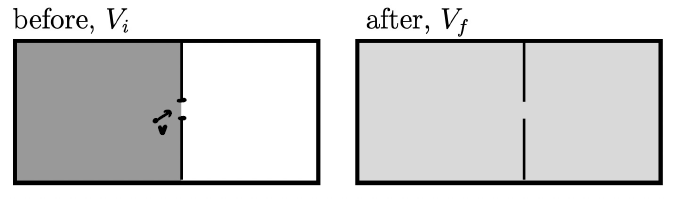
\includegraphics[width=100mm]{31.png}
\end{figure}

Since the system is insulated, total heat flowing in is $Q=0$. The work done on the system is $W=0$ since the system is isolated and there is no change in volume of the box. According to the first law of thermodynamics, $\Delta U=0$\footnote{Here is another way to see why it is true: For monoatomic gas particles, its internal energy is just its kinetic energy. There is nothing in the expansion process that changes molecule kinetic energies, so there is no internal energy change.}. Also since the gas is ideal, its internal energy depends on temperature only, so $\Delta T=0$\footnote{If the gas is not ideal, this is not necessarily true. For real gases, internal energy is constant but temperature is not. The internal energy of a real gas depends on both temperature and pressure. So, if $U$ remains constant and pressure changes, the temperature must change.}. \\

The pressure of the gas is changing, since it is expanding throughout the whole box. To see it more explicitly, consider the ideal gas law $PV=Nk_BT$. We know that temperature is constant $T_i=T_f$, this means

\[P_iV_i=P_fV_f\]

So, if the gas expands in the box that is twice the gas's volume, its pressure will be halved. \\

The free expansion is irreversible process since it produces entropy. Suppose the compartments in the box is divided equally. Let $\Omega$ denote the number of ways to place ideal gas particles in the box. For a single gas particle, before expansion it can only reside in the left compartment, so $\Omega_i=1$. After expansion, it can reside in either the left or right compartment, so $\Omega_f=2$. For $N$ gas particles, before expansion: $\Omega_i=1^N$ and after expansion: $\Omega_f=2^N$. Applying the statistical definition of entropy, the total entropy change during the free expansion for $N$ particles is:

\[\Delta S=k_B\ln\Omega_f-k_B\ln\Omega_i=k_B\ln\left(\frac{\Omega_f}{\Omega_i}\right)=k_B\ln(2^N)=Nk_B\ln(2)\]

Alternatively, we can apply the first thermodynamic identity $dU=TdS-PdV=0$ to calculate the entropy as follows:

\[\Delta S=\int dS=\int \frac{P}{T} dV=\int_{V_i}^{V_f} \frac{Nk_B}{V} dV=Nk_B\ln\left(\frac{V_f}{V_i}\right)=Nk_B\ln(2)\]

assuming the expansion happens quasistatically. In quasistatic expansion, the gas expands by a very small amount $\delta V$. After thermal equilibrium is reached, we then let the gas undergo another free expansion by $\delta V$ and wait until thermal equilibrium is reached. We repeat this until the volume reaches $V_f$.

\subsection{Entropy of Ideal Gas}

There exists a closed formula for calculating the entropy of ideal gas. To derive it, we start with the first thermodynamic identity:

\[dU=TdS-PdV\]

We rearrange terms a bit:

\[dS=\frac{1}{T}dU+\frac{P}{T}dV\]

Then we apply the ideal gas law $PV=Nk_BT$ and the thermal energy relation $U=\frac{f}{2} Nk_BT$:

\[dS=\frac{f}{2}\frac{Nk_B}{U}dU+\frac{Nk_B}{V}dV=Nk_B\left[ \frac{f}{2}\frac{dU}{U}+\frac{dV}{V} \right]\]

Next, we integrate both sides to get:

\[S(U,V,N)=Nk_B\left[ \frac{f}{2}\ln(U)+\ln(V) \right]+f(N)=Nk_B\ln\left(VU^\frac{f}{2}\right)+f(N)\]

where $f(N)$ is an integration constant with respect to the variables $U$ and $V$ and it only depends on $N$. To determine the constant, we use the fact that entropy is supposed to be an extensive property. In other words, if a system is $\alpha$ times larger (ie. $U,V,N$ is $\alpha$ times larger) then its entropy is $\alpha$ times larger. That is,

\[S(\alpha U,\alpha V,\alpha N)=\alpha S(U,V,N)\]

We have

\[S(\alpha U,\alpha V,\alpha N)=\alpha Nk_B\ln\left(VU^\frac{f}{2} \alpha^{1+\frac{f}{2}}\right)+f(\alpha N)\]

and

\[\alpha S(U,V,N)=\alpha Nk_B\ln\left(VU^\frac{f}{2}\right)+\alpha f(N)\]

Applying the relation $S(\alpha U,\alpha V,\alpha N)=\alpha S(U,V,N)$ gives:

\[\alpha Nk_B\ln\left(\alpha^{1+\frac{f}{2}}\right)+f(\alpha N)=\alpha f(N)\]

To find $f(N)$, we let $\alpha=\frac1N$:

\[k_B\ln\left(\frac{1}{N^{1+\frac{f}{2}}}\right)+f(1)=\frac{f(N)}{N}\]

\[f(N)=-Nk_B\ln\left(N^{1+\frac{f}{2}}\right)+Nf(1)\]

We let the value of $f(1)$ to be $k_Bc$, where $c$ is some constant, for aesthetic reasons\footnote{$f(1)$ can't be $k_Bc+b$ because it will not make entropy extensive.}:

\[f(N)=-Nk_B\ln\left(N^{1+\frac{f}{2}}\right)+Nk_Bc\]

Substituting our $f(N)$ into the entropy equation gives:

\[S(U,V,N)=Nk_B\ln\left(VU^\frac{f}{2}\right)-Nk_B\ln\left(N^{1+\frac{f}{2}}\right)+Nk_Bc\]

\[\boxed{S(U,V,N)=Nk_B\left[\ln\left(\frac{V}{N} \left(\frac{U}{N}\right)^\frac{f}{2}\right)+c\right]}\]

This equation is known as Sackur–Tetrode equation. The constant $c$ can be determined using quantum mechanics whose derivation is bit out of scope here. For monoatomic ideal gas, the constant becomes

\[c=\frac32 \ln\left( \frac{4\pi m}{3h^2} \right) + \frac52\]

where $h$ is Planck's constant and $m$ is the mass of a gas particle. The equation becomes:

\[\boxed{S(U,V,N)=Nk_B\left[\ln\left( \frac VN \left(\frac{4\pi m}{3h^2}\frac UN\right)^{\frac32}\right)+\frac52\right]}\]

Consider the free expansion of gas in the box with two equally divided compartments so that $2V_i=V_f$. We can apply Sackur–Tetrode equation to determine entropy change:

\[\Delta S=S(U,V_f,N)-S(U,V_i,N)=Nk_B\ln\left(\frac{V_f}{V_i}\right)=Nk_B\ln(2)\]

which is consistent with the result from the previous section. \\

We should note that Sackur–Tetrode equation we derived works for \textit{indistinguishable} particles only. Suppose we have a container filled with ideal gas, partitioned into two equal parts.

\begin{figure}[H]
	\centering
	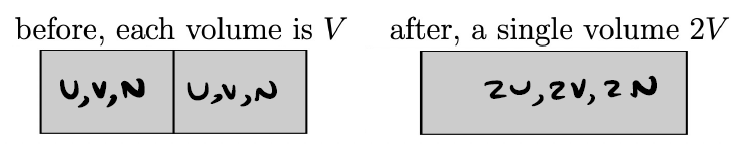
\includegraphics[width=100mm]{37.png}
\end{figure}

The entropy of the gas before the partition is removed is $2S(U,V,N)$. After removing the partition, the entropy is $S(2U,2V,2N)$. Due to the extensiveness of entropy, even if we remove the partition the entropy of the gas is the same:

\[S(2U,2V,2N)=2S(U,V,N)\]

This is only true if we have indistinguishable gas particles on both sides. The next section will deal with cases when the particles are distinguishable.

\begin{texample}
	One mole of krypton at $\SI{300}{\kelvin}$ and $\SI{1}{\atmosphere}$ is stored in a container like this:
	
	\[\underline{\overline{\begin{vmatrix} &  &  \\  & \mathrm{Krypton} &  \\  &  & \end{vmatrix} \begin{vmatrix} & & & & & & & \\ & & & \mathrm{Vacuum} & & & \\ & & & & & & & \end{vmatrix}}}\]
	
	The right-hand-side, evacuated part has $2$ times the volume of the krypton side. The wall between the two sides breaks and krypton gas fills the whole container. Assume that no energy passes through the walls. What is the entropy of the krypton gas afterwards? \\
	
	The mass of the single krypton gas particle is $m=\SI{83.798}{\atomicmassunit}=\SI{1.391e-25}{\kilo\gram}$. The number of krypton particles is $N=N_A=6.023e23$. The volume can be calculated from the ideal gas law as follows:
	
	\[V=\frac{Nk_BT}{P}=\SI{0.02463}{\meter\cubed}\]
	
	The internal energy of the gas is:
	
	\[U=\frac32 Nk_BT=\SI{3743}{\joule}\]
	
	Plugging in everything into Sackur–Tetrode equation gives:
	
	\[S(U,V,N)=Nk_B\left[\ln\left( \frac VN \left(\frac{4\pi m}{3h^2}\frac UN\right)^{\frac32}\right)+\frac52\right]=\SI{164.171}{\joule\per\kelvin}\]
	
	The entropy change after the free expansion is:
	
	\[\Delta S=S(U,3V,N)-S(U,V,N)=Nk_B\ln(3)=\SI{9.138}{\joule\per\kelvin}\]
	
	The entropy of the krypton gas after the free expansion is therefore:
	
	\[S=\SI{164.171}{\joule\per\kelvin}+\SI{9.138}{\joule\per\kelvin}=\SI{173.31}{\joule\per\kelvin}\]
\end{texample}

\subsection{Entropy of Mixing}

Suppose we have a container partitioned into two parts of equal volume $V$. Each compartment is filled with a different type of ideal gas (each has $N$ atoms and $U$ internal energy).

\begin{figure}[H]
	\centering
	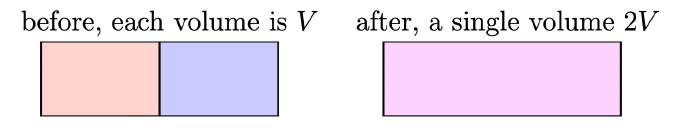
\includegraphics[width=100mm]{38.png}
\end{figure}

When we remove the partition, the entropy increases. Applying Sackur–Tetrode equation gives:

\[\Delta S=2S(U,2V,N)-2U(U,V,N)=2Nk_B\ln\left(\frac{2V}{V}\right)=2Nk_B\ln(2)\]

In fact, when you mix two different gases of identical internal energy, volume and amount of particles, the entropy increase is always $\Delta S=2Nk_B\ln(2)$. \\

We can also prove this by counting. Suppose the number of microstates in the left and right partition is given by $\Omega_d$ each, assuming that both partitions contains $N$ \textit{distinguishable} particles each. But since all particles in each partition are of one kind, the number of microstates in each partition becomes $\Omega=\frac{\Omega_d}{N!}$ where the factor $N!$ is used to prevent overcounting of duplicate microstates. The total number of microstates of the whole container before the partition is removed is:

\[\Omega_i=\frac{\Omega_d}{N!}\frac{\Omega_d}{N!}=\frac{\Omega_d^{tot}}{(2N)!}\]

where $\Omega_d^{tot}$ is the number of microstates of the whole container, assuming that \textit{all} particles are distinguishable. When the partition is removed, the total number of microstates becomes:

\[\Omega_f=\frac{\Omega_d^{tot}}{N!N!}\]

we divide $\Omega_d^{tot}$ by $N!$ twice since there are two kinds of particles. The entropy change is:

\[\Delta S=k_B\ln\Omega_f-k_B\ln\Omega_i=k_B\ln\left(\frac{(2N)!}{(N!)^2}\right)\]

Next, we apply Stirling's approximation $\ln N!\approx N\ln N-N$ which gives:

\[\Delta S=k_B\left[ \ln\left((2N)!\right)-2\ln(N!) \right]=k_B\left[ 2N\ln(2N)-2N-2N\ln(N)+2N \right]=2Nk_B\ln(2)\]

as expected.

\begin{texample}
	Two moles of argon and a mole of neon each is stored side by side at $\SI{300}{\kelvin}$ and $\SI{1}{\atmosphere}$:
	
	\[\underline{\overline{ \begin{vmatrix} &  &  \\  & \mathrm{Ar} &  \\  &  & \end{vmatrix} \begin{vmatrix} &  &  \\  & \mathrm{Ar} &  \\  &  & \end{vmatrix} \begin{vmatrix} &  &  \\  & \mathrm{Ne} &  \\  &  & \end{vmatrix} }}\]
	
	How much will the entropy of this system increase if the barriers are removed and those two gases are allowed to mix freely? \\
	
	The extensive variables for neon gas are $U,V,N$ and for argon gas are $2U,2V,2N$ since the amount of argon is twice that in neon. The initial entropy before the barriers are removed is:
	
	\[S_i=S(2U,2V,2N)+S(U,V,N)\]
	
	After the barriers are removed:
	
	\[S_f=S(2U,3V,2N)+S(U,3V,N)\]
	
	The total entropy change is therefore:
	
	\begin{align*}
		\Delta S&=S(2U,3V,2N)+S(U,3V,N)-S(2U,2V,2N)-S(U,V,N) \\
		&=Nk_B\left[2\ln\left(\frac{3V}{2N}\right)+\ln\left(\frac{3V}{N}\right)-2\ln\left(\frac{2V}{2N}\right)-\ln\left(\frac{V}{N}\right)\right] \\
		&=Nk_B\left[2\ln\left(\frac{3}{2}\right)+\ln\left(3\right)\right] \\
		&=Nk_B\ln\left(\frac{27}{4}\right) \\
		&=\SI{15.88}{\joule\per\kelvin}
	\end{align*}
\end{texample}

\subsection{Einstein Solid}

We will study entropy of Einstein solids. The Einstein solid models a solid as a large collection of identical quantum harmonic oscillators. The energy levels in each harmonic oscillator are quantized and they are equally spaced by $hf$ energy unit. It is a useful for examining the energy distribution in a solid.

\begin{figure}[H]
	\centering
	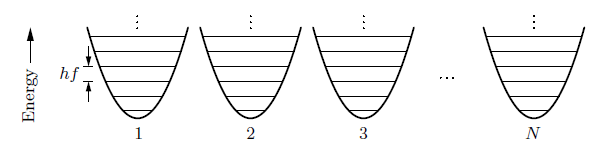
\includegraphics[width=100mm]{39.png}
	\caption{Einstein Solid with $N$ Harmonic Oscillators}
\end{figure}

Quantum harmonic oscillators are commonly used to study vibrations in solid. If there are $N$ harmonic oscillators in a 3D solid, since each atom independently move in three directions, there are $N/3$ atoms. \\

Suppose we have $q$ units of energy that needs to be distributed among $N$ harmonic oscillators. All energy levels in each oscillators are equally probable. If $N=3$ and $q=2$, the microstates are:

\begin{center}
	\begin{tabular}{|c|c|c|}
		\hline
		Energy in HO 1 & Energy in HO 2 & Energy in HO 3 \\
		\hline
		1 & 1 & 0 \\
		\hline
		1 & 0 & 1 \\
		\hline
		0 & 1 & 1 \\
		\hline
		2 & 0 & 0 \\
		\hline
		0 & 2 & 0 \\
		\hline
		0 & 0 & 2 \\
		\hline
	\end{tabular}
\end{center}

There are $6$ microstates in total. To derive the general formula for calculating the number of microstates with $N$ harmonic oscillators and $q$ energy units, suppose a energy unit is represented by a black dot and boundary between harmonic oscillators is represented by vertical bars. The below shows a microstate of an Einstein solid with $N=4$ oscillators and $q=8$ energy units:

\begin{figure}[H]
	\centering
	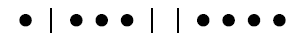
\includegraphics[width=100mm]{40.png}
\end{figure}

Any permutation of these $11$ symbols corresponds to a microstate. In general, for $N$ harmonic oscillators and $q$ energy units, there are $N+q-1$ symbols in total with $q$ black dots and $N-1$ vertical bars. The number of permutations is:

\[\Omega(N,q)={N+q-1 \choose q}\]
